\section{SA³: Semantic Activity Annotation}
\label{sec:clustering:sa3}

%Brief introduction to the algorithm:
%- Inspired in knowledge-driven techniques, specially in Chen's work
%- It is not activity recognition, but offline annotation
The annotation algorithm presented in this paper is inspired in knowledge-driven activity recognition methods, specially in \cite{Chen2012a}. Three important concepts from that work are extracted and used for the presented approach:

\begin{itemize}
 \item \textbf{Domain knowledge allows recognizing activities reliably:} in contrast with data-driven techniques, which use intensively annotated datasets in order to learn activity models for recognition, knowledge-driven techniques use expert domain knowledge to model activities. Those models can be reliably used for activity recognition
 \item \textbf{Sensor activations are linked to user-object interactions:} if a contact sensor installed in a cup changes its state, the object is assumed to be used for an activity. Sensors' information is modelled to allow transformations from sensor activations to user-object interactions or \textbf{actions}. Following with the contact sensor of the cup, whenever an activation is received, it is interpreted as an action, which can be named as \textit{hasContainer(cup)}
 \item \textbf{Activities can be modelled as sequences of actions:} even though richer information can be provided as location and time, to keep activity models as simple as possible, we only consider necessary actions. As such, the \textit{MakeCoffee} activity can be modelled as the action sequence \textit{\{hasContainer(x), hasCoffee(y)\}}.
\end{itemize}

Real-time activity recognition needs complete activity models to have a reliable recognition performance. However, providing complete activity models is very complicated, since each user executes varied action sequences to perform the same activity. For example, to make a coffee, some users may use milk and sugar, while others may add only some cream. But making coffee will always imply using coffee and having a container, i.e. the action sequence \textit{\{hasContainer(x), hasCoffee(y)\}}. This prior knowledge is used in $SA^3$ for activity annotation.

Activity annotation and recognition is not the same thing. Activity annotation can make use of the whole dataset offline, with no time restrictions. On the other hand, activity recognition is required to work while activities are being performed, so only past sensor activations can be used. This key difference makes feasible using incomplete activity models to annotate activities, in contrast with the real-time recognition problem.

\subsection{Basic Concepts}
%- Explain what sensor activations and actions are (ontologies could be good to represent that knowledge, but we do not use them at this moment to make the tool lighter)
%- Explain minimal activity models (action patterns + maximum duration) (once again, ontology issues)
%- Time-stamped sensor activation dataset (show a sample and explain)
\begin{itemize}
 \item \textbf{Sensor activations (SA):} it is assumed that environments are equipped with sensors that can collect information about user-object interactions. Whenever those sensors change their states, a sensor activation is collected. Sensor activations are then composed by a sensor identifier and a time-stamp
 \begin{equation*}
  SA = \{time\text{-}stamp, sensorID\}
 \end{equation*}
 \item \textbf{Sensor dataset:} a time-ordered sequence of sensor activations
 \item \textbf{Actions:} actions are the primitives of activities and are directly linked to sensor activations. The link between sensor activations and actions is manually established. Tables are used where several sensor activations are linked to an action. For example, \textit{cupObjSensor} and \textit{glassObjSensor} are linked to the action \textit{hasContainer}. A sensor activation can only be linked to one single action. The transformation function is defined as:
 \begin{equation*}
  Trans(SA) : SA \rightarrow Action
 \end{equation*}

 \item \textbf{Action dataset:} a time-ordered sequence of actions
 \item \textbf{Minimal activity models:} activity models are sequences of actions defined by a domain expert. Minimal activity models refer to the minimal number of necessary actions to perform an activity. The objective of such models is to represent incomplete but generic activity models which provide enough information to detect activities. Minimal activity models also have an estimation of the maximum duration of the activity based on a heuristic %That duration estimation turned to be essential for robust annotation in noisy scenarios
 \begin{equation*}
  Activity_n = \{action_a, action_b, \ldots , max\_duration\}
 \end{equation*}

\end{itemize}


\subsection{SA³: Semantic Activity Annotation Algorithm}
%- Maybe having a name for the tool could be nice -> SA3 ?
%- Explain the three-step algorithm
%- Show pseudo-code for the algorithm

Having as inputs a sensor dataset, sensor-action transformation functions and minimal activity models, the objective of $SA^3$ is to generate an annotated sensor dataset, where each sensor activation will have an activity label or the special label \textit{None}, which represents lack of known activity. Single-user single-activity scenarios are considered, so no interleaved activities will be in the sensor dataset. Considering those constraints, a three-step algorithm has been designed:

\begin{enumerate}
 \item \textbf{Sensor-action transformation step:} the first step takes as input the sensor dataset and transformation functions to generate an action dataset. For each sensor activation in the sensor dataset, the transformation function is applied to obtain the corresponding action. In consequence, a sensor sequence such as:
 \begin{equation*}
 \begin{split}
   \{cupObjSensor, whiteSugarSensor, skimmedMilkSensor\}
 \end{split}  
 \end{equation*}
 will be transformed to:
 \begin{equation*}
 \begin{split}
  \{hasContainer(cup), hasFlavour(white\text{-}sugar), hasMilk(skimmed\text{-}milk)\}
 \end{split}   
 \end{equation*}
 
Since only actions and not objects are relevant for activity annotation, \textit{hasContainer(cup)} will be used as \textit{hasContainer} 

 \item \textbf{Activity sequence finding step:} all the occurrences of minimal activity models are found iterating on the action dataset. For an action pertaining to a minimal activity model following actions are searched. Those actions are considered to describe the activity if two criteria are fulfilled: 
 \begin{enumerate}
  \item \textit{Completion criterion}: the action sequence has to contain all the actions of the corresponding minimal activity model
  \item \textit{Duration criterion}: the duration of the action sequence has to be smaller than the duration estimation of the corresponding minimal activity model
 \end{enumerate}
 Depending on the activity models, the actions dataset and noise levels, detected activities can overlap each other. Here is an illustrative example, where time-stamps are ignored since duration criterion is satisfied. Imagine we define minimal activity models for \textit{MakeCoffee, MakeTiramisu, MakeWhippedCream} and \textit{BrushTeeth}, where:
 \begin{equation*}
  \begin{split}
   MakeCoffee =\{hasCoffee, hasContainer, hasFlavour\} \\
  MakeTiramisu = \{hasCream, hasContainer, hasCoffee\} \\
  MakeWhippedCream = \{hasFlavour, hasContainer, hasCream\} \\
  BrushTeeth = \{hasBrusher, hasToothPaste, turnOnTap\} 
  \end{split}
 \end{equation*} 
 
Let us consider the following action sequence from the action dataset:
\begin{equation*}
\begin{split}
 \{hasContainer, hasCream, useCookingUtensil, hasFlavour, hasBrusher, \\ 
 hasCoffee, hasToothPaste, hasContainer, turnOnTap\}
\end{split}  
\end{equation*}
Figure \ref{fig:overlap} shows all the activities found applying the completion and duration criterion. Activities overlap each other, because there are several actions that belong to several activities. Notice also that there are some actions that are not in any activity model, which is totally feasible for our approach.
\begin{figure}[htbp]
\centering
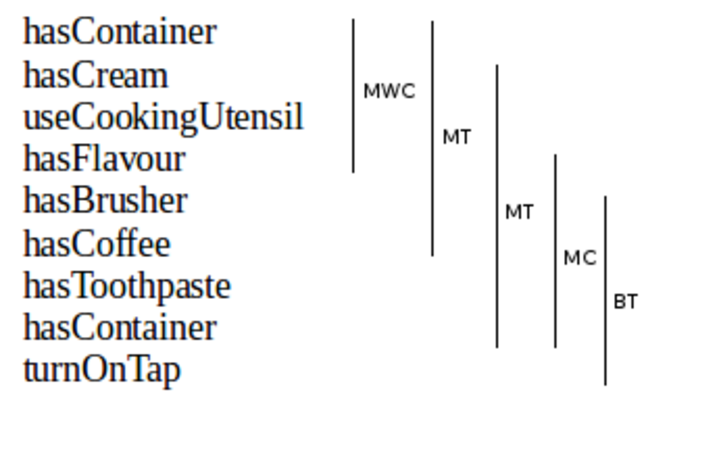
\includegraphics[width=\textwidth]{overlapping_activities.pdf}
    \caption{Illustrative example of the output of the step 2 of $SA^3$. MWC refers to \textit{MakeWhippedCream}, MT to \textit{MakeTiramisu}, MC to \textit{MakeCoffee} and BT to \textit{BrushTeeth}}
    \label{fig:overlap}
\end{figure}

\item \textbf{Correct activity sequence fitting step:} having the overlapping activities, the objective of this step is to find the maximum number of activities that do not overlap. This heuristic is derived from the fact that only none interleaved activities are considered. Applying it, the example of Figure \ref{fig:overlap} can be solved appropriately. The solution found by the algorithm is that there are only two activities in that action sequence:
\begin{equation*}
  \begin{split}   
  MakeWhippedCream = \{hasContainer, hasCream, useCookingUtensil, hasFlavour\} \\
  BrushTeeth = \{hasBrusher, hasCoffee, hasToothPaste, hasContainer, turnOnTap\} 
  \end{split}
 \end{equation*}  

Hence, \textit{hasCoffee} is probably due to a faulty sensor activation and \textit{hasContainer} may refer to a glass used in the bathroom to rinse the mouth. 
\end{enumerate}

This three-step algorithm is depicted as pseudo-code in Algorithm \ref{alg:sa3}. It has been designed to work with noisy sensor activations, varying order for activity executions and sensor activations that do not belong to any activity model. That flexibility allows using the tool in many different datasets. Section \ref{evaluation} contains many cases to show the performance of the algorithm in several demanding situations.

\begin{algorithm}
 \caption{$SA^3$ algorithm for semantic activity annotation}
 \label{alg:sa3}
 \begin{algorithmic}
 \REQUIRE sensor\_dataset, transformation\_function, minimal\_activity\_models
 \ENSURE annotated\_dataset
 \STATE $action\_dataset \leftarrow apply\_transform\_function(sensor\_dataset, transformation\_function)$
 \FORALL{$action \in action\_dataset$}
  \IF{$action \in minimal\_activity\_models$}    
    \STATE $activities \leftarrow obtain\_activities(action, minimal\_activity\_models)$
  \ENDIF
  \FORALL{$activity \in activities$}
    \STATE $// \text{ Use duration and completion criteria}$
    \STATE $detected\_activities \leftarrow find\_proper\_activities(minimal\_activity\_models)$
  \ENDFOR
 \ENDFOR
 \STATE $annotated\_dataset \leftarrow find\_non\_overlapping\_activities(detetected\_activities)$
 \RETURN $annotated\_dataset$
 \end{algorithmic}
\end{algorithm}
